\documentclass[11pt,a4paper,oneside]{article}
\usepackage[UTF8,adobefonts]{ctex}

\usepackage{wrapfig}
\usepackage{indentfirst}
\usepackage{amsmath}
\usepackage{float}
\usepackage{ulem}
\usepackage[top=1in,bottom=1in,left=1.25in,right=1.25in]{geometry}

\usepackage{color}
\usepackage{xcolor}

\usepackage{multirow}

\begin{document}

\begin{figure}[H]
 \centering
  
\includegraphics[width=13cm]{表头.png}
\end{figure}
\begin{center}
\textbf{{\large 实验名称:\uline{         薄透镜和单球面镜焦距的测量       }}}
\end{center}

\section*{一、实验目的}
\begin{enumerate}
\item 掌握简单光路的调整方法——等高共轴调整。
\item 掌握几种常用的测量薄透镜焦距的基本方法。
\item 掌握不同测量方法中消除系统误差或减小随机误差的方法。
\item 掌握测量单球面镜焦距的简单方法。
\end{enumerate}

\section*{二、实验原理}
薄透镜是指透镜中心厚度d远小于焦距f的透镜。近轴光线是指通过透镜中心部分并与主光轴夹角很小的一部分光线。为了满足近轴光线的条件,常在透镜前加一带孔的主屏,即光阑,以挡住边缘光线;同时选用小物体,并做等高共轴调节,使入射光线与主轴夹角很小。紫近轴光线条件下,薄透镜成像规律用下式表示:
\begin{center}
$\displaystyle\frac{1}{u}+\displaystyle\frac{1}{v}=\displaystyle\frac{1}{f}$
\end{center}
式中,u为物距,实物为正,虚物为负;v为像距,实像为正,虚像为负;f为焦距,凹透镜为负,凸透镜为正。

对于单球面镜,半径为r的单球面镜焦距与曲率半径关系如下:
\begin{center}
$f=\displaystyle\frac{r}{2}$
\end{center}

\subsection*{实验1.物距相距法测量透镜焦距}

\subsubsection*{(1)物距像距法测凸透镜的焦距}
物体发出的光经过凸透镜折射后将成像在凸透镜的另一侧,将测出的物距和相距带入透镜成像公式。

\subsubsection*{(2)物距像距法测凹透镜焦距}
由于凹透镜是发散透镜,对实物成虚像,所以直接测量凹透镜的物距、像距,难以两全。为了测量凹透镜的焦距,我们只能借助与凸透镜成一个倒立的实像作为凹透镜的虚物,虚物的位置可以测出。凹透镜能对虚物成实像,实像的位置可以测出,使能得到能用像屏接收的实像。其测量原理如下光路图所示:

\begin{figure}[H]
 \centering
  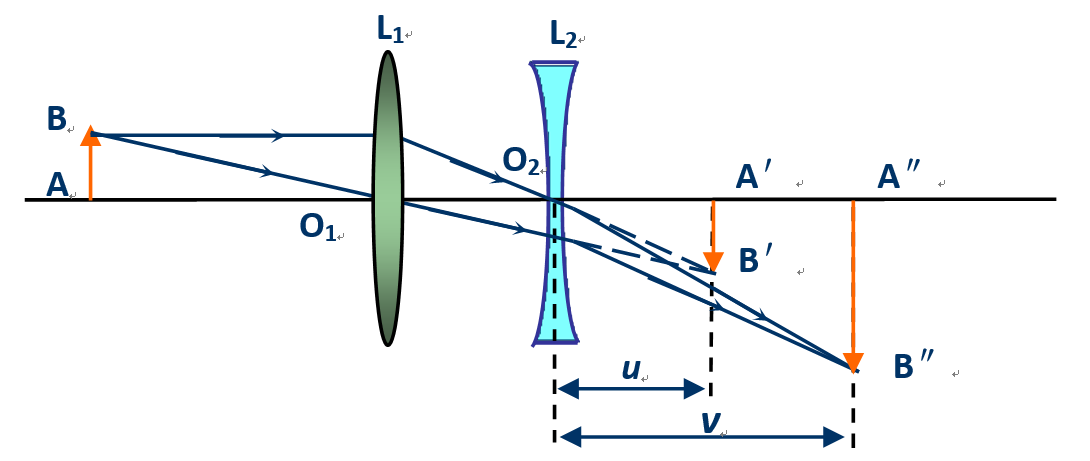
\includegraphics[width=12cm]{10612.png}
\end{figure}

实物AB经凸透镜$L_1$成像于A'B'。在$L_1$和A'B'之间插入待测凹透镜$L_2$,就凹透镜$L_2$而言,虚物A'B'又成像于A''B''。实验中,调整$L_2$及像屏至合适的位置,就可找到透镜组所成的实像A''B''。因此可把$O_2A'$看为凹透镜的物距u,$O_2$A''看为凹透镜的像距v,则由成像公式可得:
\begin{center}
$f=\displaystyle\frac{{u_2}{v_2}}{{u_2}+{v_2}}$
\end{center}
\subsection*{实验2.自准直法测透镜焦距}

\subsubsection*{(1)自准直法测凸透镜焦距}
当小孔A处于透镜L的前焦距面时,光经过透镜成为平行光,若在此平面平行光的光路上放一个平面镜垂直于平行光,经平面镜反射再经透镜后成像于原物P 处(记为Q)。因此,P 点到透镜中心O 点的距离就是透镜的焦距f。其像在与光孔对称的位置上。与光源等大反向。
\subsubsection*{(2)自准直法测凹透镜焦距}
因为凹透镜是发散透镜,所以要由它获得一束平行光,必须借助于一个凸透镜才能实现。

首先由透镜L1将小孔成像在S’处,然后将透镜后面,成像前面依次放上凹透镜,平面镜。移动凹透镜,当凹透镜焦点和凸透镜焦点重合时,平面镜将接受到垂直于其的平行光,反射后经原路返回,在小孔旁成等大反向的像。于是确定了像点和凹透镜光心的位置就可以确定凹透镜的焦距f。
\subsection*{实验3.共轭法测量凸透镜焦距}
设凸透镜的焦距为f,使物与屏的距离L>4f并保持不变。移动透镜至$x_1$处,在屏上呈放大实像,再移动到$x_2$处,成缩小实像。令$x_1$和$x_2$间的距离为a。物到像屏的距离为b,根据共轭关系有$u_2=v_1$,$u_1=v_2$由物距像距与焦距的关系,可以导出公式:
\begin{center}
$f=\displaystyle\frac{b^{2}-a^{2}}{4b}$
\end{center}
实验测出a和b,就可以求出f。

\subsection*{实验4.自准直法测量球面镜焦距}
\subsubsection*{(1)自准直法测凹面镜的焦距}
将待测凹面镜置于光源附近与物一定距离处,直到在原物的位置旁边出现等大反向的实像为止。记录下此时凹面镜的位置,它与物的距离就是待测凹面镜的曲率半径,进而算出焦距。
\subsubsection*{(2)自准直法测凸面镜的焦距}
因为凸面镜是发散镜,所以要由它获得一束平行光,必须借助于一个凸透镜才能实现。
首先由透镜L1将小孔成像在S’处,然后将透镜后面,成像前面放上凸面镜。移动凸面镜,当凸面镜焦点和凸透镜焦点重合时,凸面镜将反射经原路返回的光,在物旁成等大反向的像。于是确定了像点和凸面镜光心的位置就可以确定凹透镜的曲率半径r,进而算出焦距。

\section*{三、实验仪器}
光具座、不同焦距凹透镜、凸透镜若干,光源、屏、箭状孔、小孔、平面反射镜等

\section*{四、实验步骤}
成像法测量焦距的所有试验中,由于人眼对于“清晰”的判断不准确,故使用以下方法:
\begin{enumerate}
\item 从左向右移动透镜时,当第一次成清晰像时候记下该处的位置;
\item 继续向右移动,至像刚好开始不清晰,记下此处位置;
\item 将透镜再往左一点从右向左移动透镜,依照1、2相似的步骤记录两个位置。
\item 将四个数求平均,就是需要的位置。
\end{enumerate}

另外,为了减少支架中心与透镜中心位置不重合的误差,采用对称测量法,在测完一组数据后,将透镜反转180度再测一组。

\subsection*{实验1.物距像距法测透镜焦距}
\subsubsection*{(1)物距像距法测凸透镜的焦距}
\begin{enumerate}
\item 物体发出的光经过凸透镜折射后将成像在凸透镜的另一侧成清晰的像,记下此时透镜、屏和物体的位置。
\item 分别在f<u<2f、u=2f、u>2f测出像距和物距。
\end{enumerate}

\subsubsection*{(2)物距像距法测凹透镜焦距}
\begin{enumerate}
\item 将屏、辅助透镜和屏照光路图放在光具座上,是屏和物体的距离里大于4f。移动透镜使屏上呈清晰的像。固定透镜并记录位置。
\item 将待测凹面镜放在屏和凸透镜之间,移动屏,至屏上出现清晰的像。固定屏,细调凹透镜至像最清晰。记录凹透镜与屏的位置。
\end{enumerate}

\subsection*{实验2.自准直法测透镜焦距}
\subsubsection*{(1)自准直法测凸透镜焦距}
\begin{figure}[H]
 \centering
  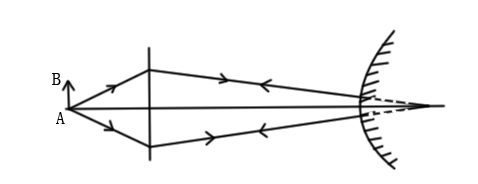
\includegraphics[width=8cm]{自准直法测凸面镜焦距.png}
\end{figure}
注意:
\begin{enumerate}
	\item 要记录原始刻度
	\item 物支架刻线与小孔不重合,两者间修正值$\delta$
	\item 要采用对称测量法消除系统误差
\end{enumerate}

\subsubsection*{(2)自准直法测凹透镜焦距}
\begin{figure}[H]
 \centering
  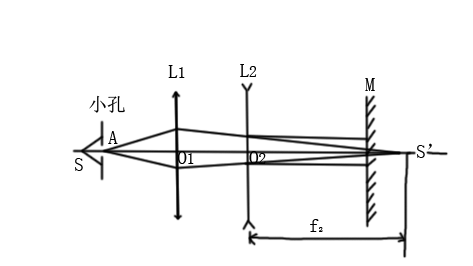
\includegraphics[width=8cm]{自准直测凹透镜.png}
\end{figure}
注意:
\begin{enumerate}
	\item 物通过凸透镜和凹透镜后成像暗
	\item 应保持物屏和凸透镜的位置不变,重复多次
\end{enumerate}

\subsection*{实验3.共轭法测凸透镜焦距}
\begin{figure}[H]
 \centering
  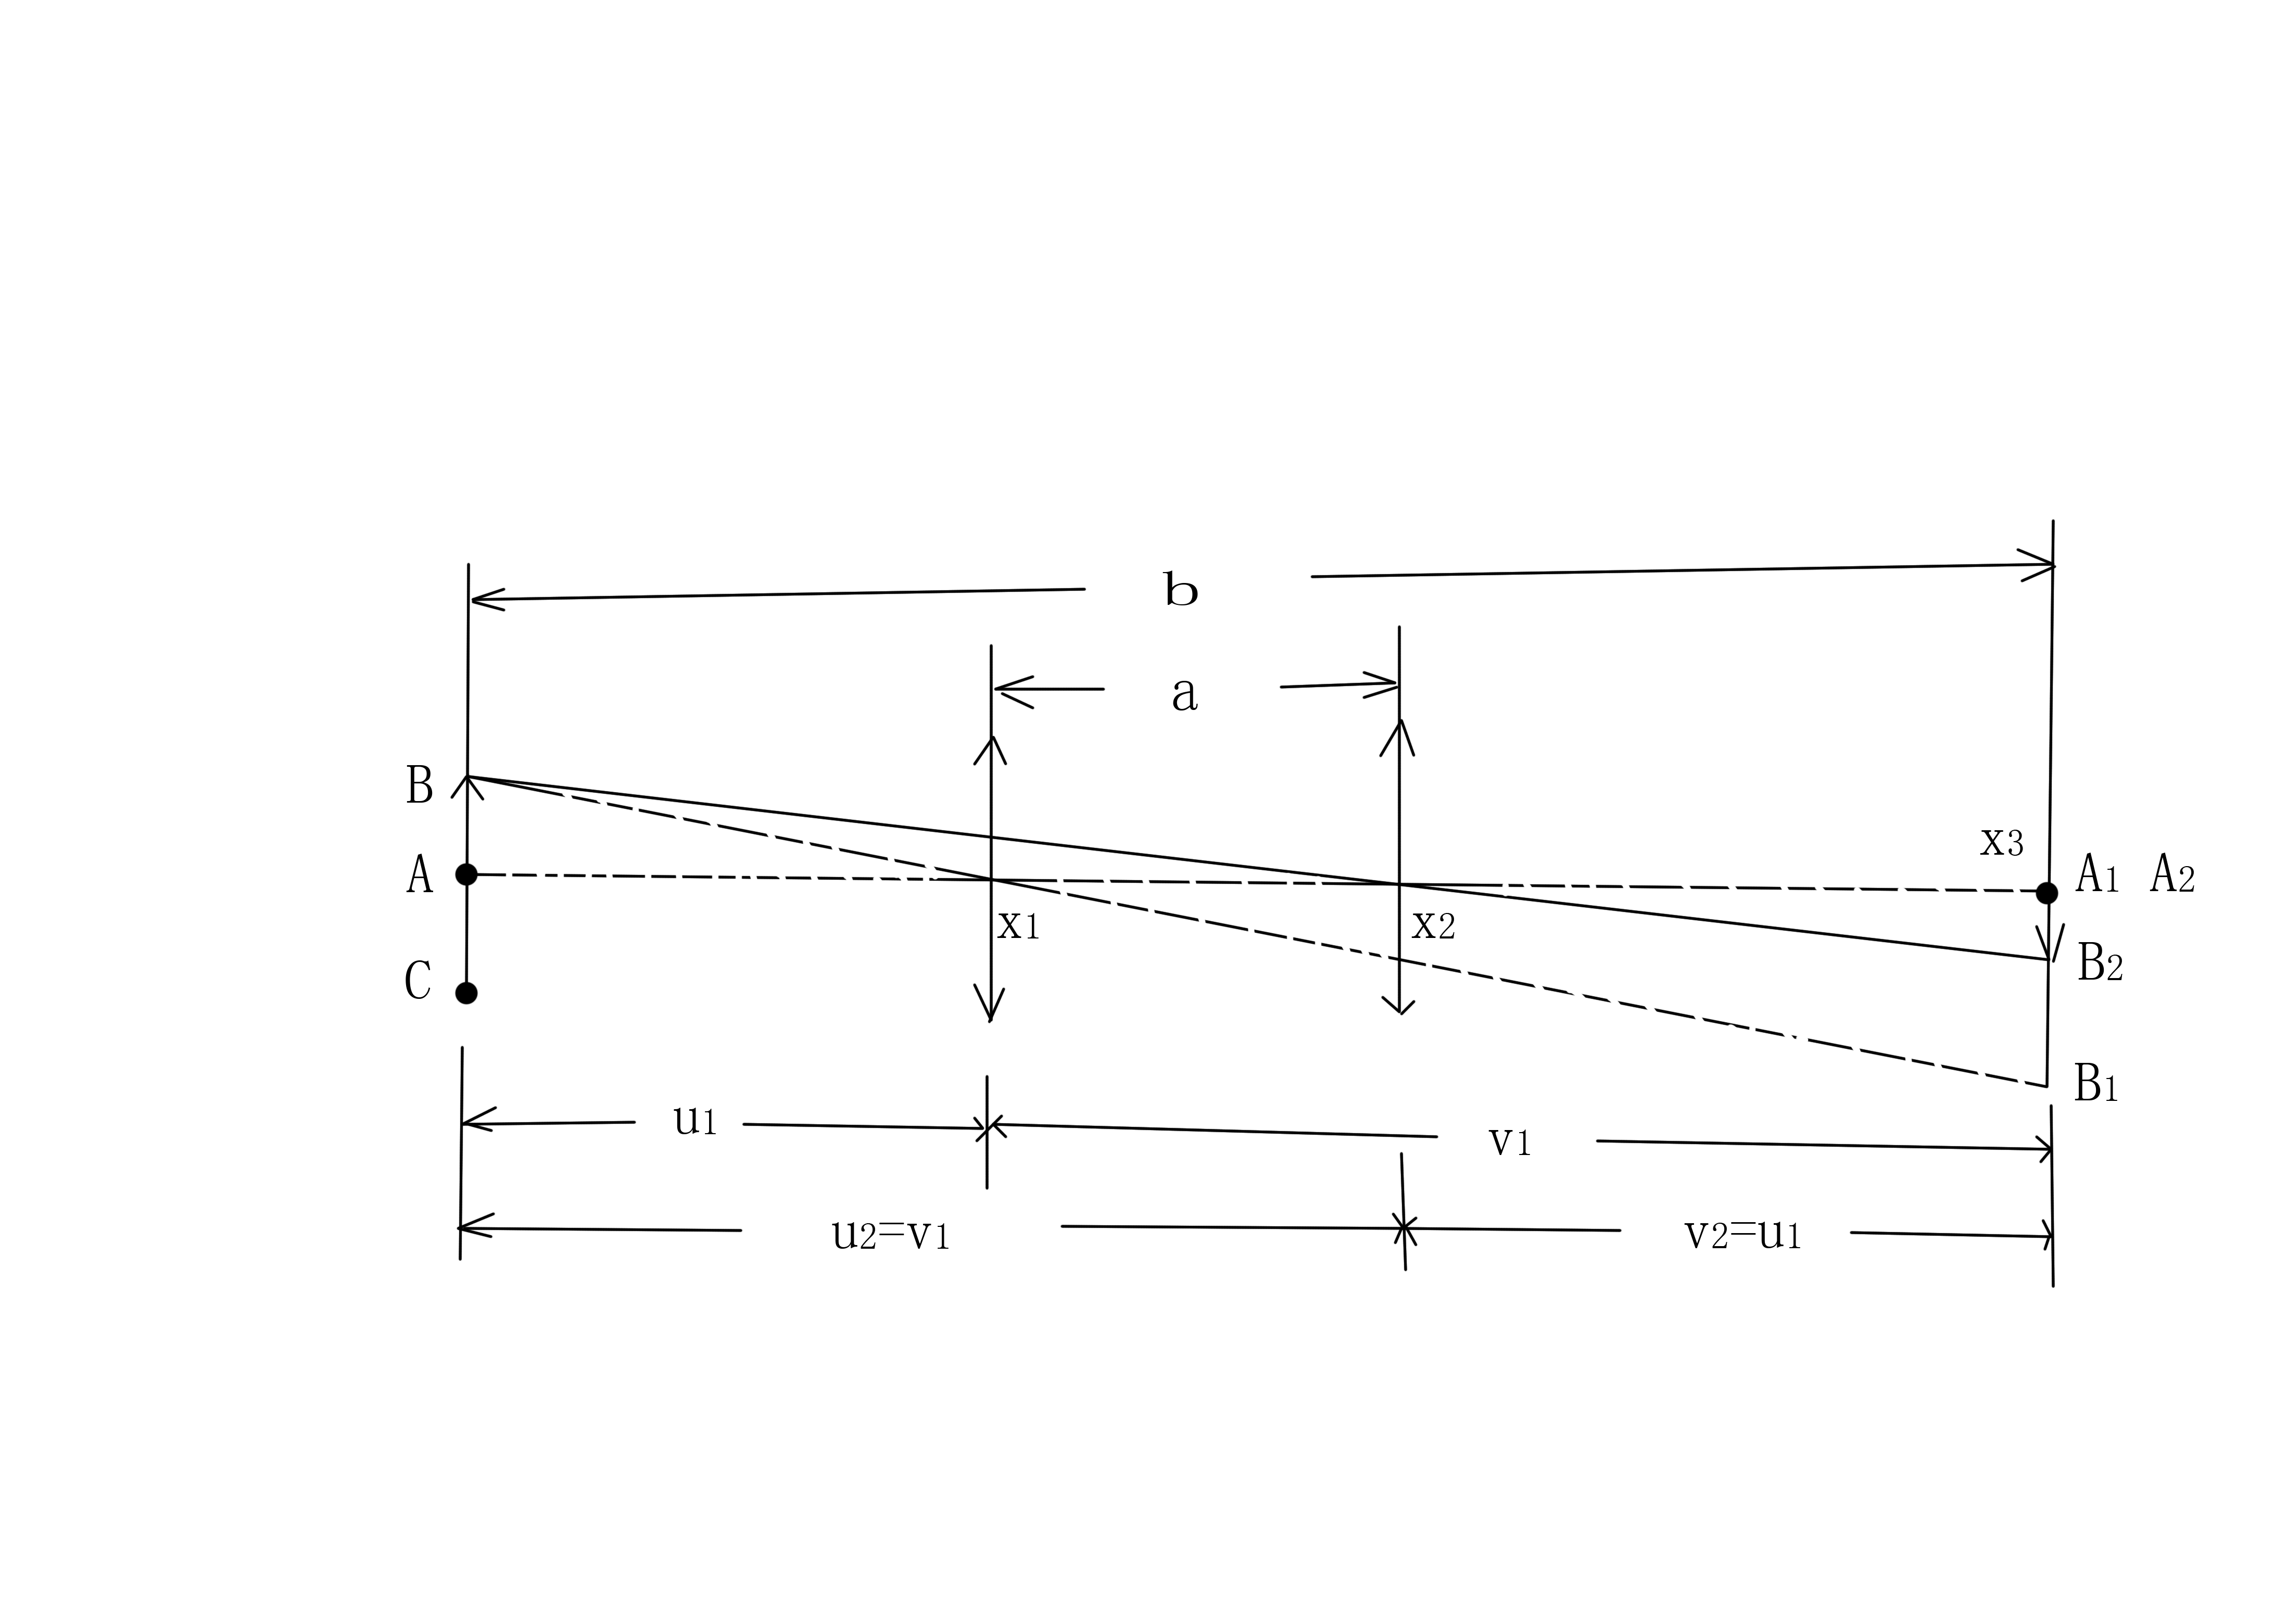
\includegraphics[width=12cm]{共轭法测凸透镜焦距.png}
\end{figure}
\begin{enumerate}
\item 查看焦距的大致焦距f,如光路图所示摆放光具,使物与屏的距离L>4f并保持不变;记录物和屏的位置。
\item 移动透镜至处,在屏上呈放大实像,记录凸透镜位置。
\item 移动透镜至x2处,在屏上成缩小实像,记录凸透镜位置。
\item 利用公式计算凸透镜焦距。
\end{enumerate}

$$f = \displaystyle\frac{b^2-a^2}{4b}$$

\subsection*{实验4. 自准直法测球面镜焦距}

\subsubsection*{(1)自准直法测凹面镜的焦距}
\begin{figure}[H]
 \centering
  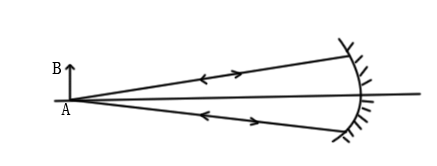
\includegraphics[width=8cm]{自准直法测凹面镜焦距.png}
\end{figure}
移动凹面镜直到在原物的位置旁边出现等大反向的实像为止。记录下此时凹面镜的位置,它与物的距离就是待测凹面镜的曲率半径,进而算出焦距。

\subsubsection*{(2)自准直法测凸面镜的焦距}
\begin{figure}[H]
 \centering
  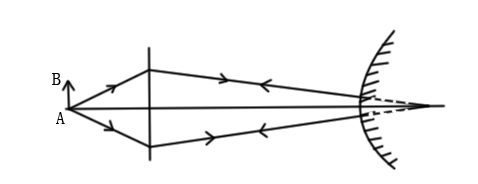
\includegraphics[width=8cm]{自准直法测凸面镜焦距.png}
\end{figure}
\begin{enumerate}
\item 按照装置图放置光学器件。
\item 移动屏幕至出现清晰的像,记录屏幕位置。
\item 然后将透镜后面,成像前面放上凸面镜。移动凸面镜至物旁成等大反向的像,记录像的位置。
\item 根据公式计算凸透镜焦距f。
\end{enumerate}

\end{document}